\section{Einf\"uhrung}

\begin{figure}[ht!]
\begin{center}
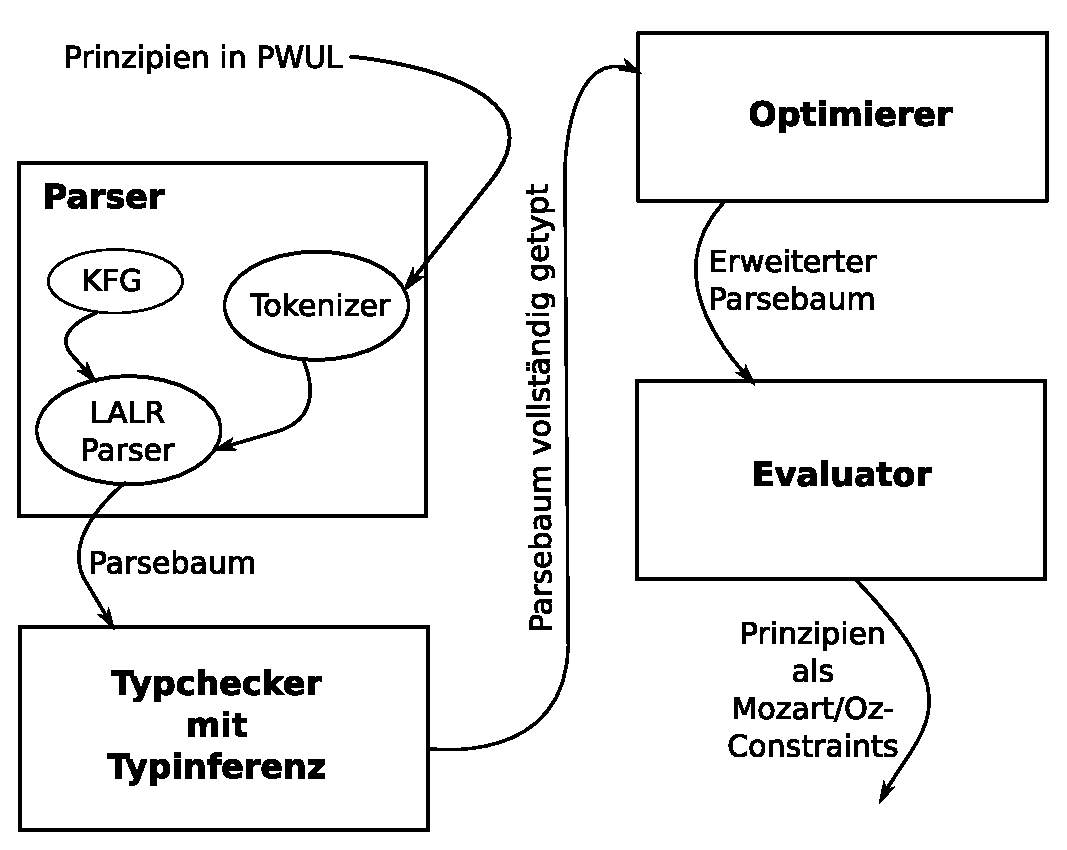
\includegraphics[width=11cm]{eps/PW_Arch.eps}
\end{center}
\caption{Architektur des PrincipleWriters}
\label{archpw}
\end{figure}

In den beiden vorherigen Kapiteln haben wir gesehen, wie Grammatiken
in XDG formalisiert werden, und mit Hilfe des XDK implementiert werden
k\"onnen. W\"ahrend der Multigraphtyp und das Lexikon analog zur XDG
Formalisierung mit Hilfe der XDK Description Language aufgeschrieben
werden konnten, konnten Prinzipien nur aus einer Bibliothek von
vordefinierten Prinzipien ausgew\"ahlt werden, oder mussten m\"uhsam
von Hand implementiert werden. Dass das blo{\ss}e Ausw\"ahlen von
Prinzipien aus der vordefinierten Prinzipienbibliothek nicht immer
reicht, haben wir anhand der CSD-Beispielgrammatik aus den beiden
letzen Kapiteln gesehen, die neben drei vordefinierten Prinzipien auch
ein Prinzip braucht, das neu implementiert werden musste. %In
%Abbildung~\ref{prinzbsp} ist dieses Prinzip, das {\tt principle.csdPW},
%in der PWUL-Syntax zu sehen.

In XDG werden Prinzipien in einer speziellen First-Order Logik
formalisiert, die einige spezielle Pr\"adikate bereitstellt, um
Constraints \"uber Multigraphen ausdr\"ucken zu k\"onnen.  Die
Prinzipien sind also logische Formeln. Zur Implementierung m\"ussen
die Prinzipien in Mozart/Oz-Mengenconstraints umgesetzt werden.  Ein
direkter Bezug zu den logischen Formeln aus XDG ist nicht
offensichtlich. Von einem Prinzipienschreiber m\"ussen also
Programmierkenntnisse in Mozart/Oz Constraintprogrammierung verlangt
werden, und um die Constraints zu optimieren, m\"ussen sogar
Expertenkenntnisse verlangt werden. Die Optimierung von Prinzipien ist
notwendig, da sie sonst wegen ihrer hohen Laufzeit nicht brauchbar
sind.

Um diese L\"ucke zwischen der Formalisierung und der Implementation zu
schlie{\ss}en wird in den n\"achsten Kapiteln die Entwicklung eines
Tools beschrieben, dem PrincipleWriter, das es Grammatikschreibern
erlaubt, Prinzipien als logische Formeln aufzuschreiben. Dazu wurde
die PrincipleWriter User Language (PWUL) entwickelt, aus der der
PrincipleWriter dann die Prinzipien in Mozart/Oz Constraints umsetzt.
Mit Hilfe der XDK Description Language und des PrincipleWriters
k\"onnen Grammatiken vollkommen analog zu ihrer Formalisierung aus XDG
in XDK implementiert werden.

\subsection{Architektur des PrincipleWriters} 

Der PrincipleWriter besteht wie in Abbildung~\ref{archpw} zu sehen ist
aus vier Komponenten:
\begin{enumerate}
\item Dem Parser, der die logische Formel zur weiteren Verarbeitung in
  die abstrakte Syntax, die eine Baumstruktur ist, bringt.
\item Einem Modul, das die fehlenden Typen inferiert, und einen
  Typchecker beinhaltet.
\item Dem Optimizer.
\item Dem Evaluator, der aus der Baumstruktur
  Mozart/Oz-Constraints erzeugt.
\end{enumerate}
Der PrincipleWriter bekommt als Eingabe eine Datei, die ein Prinzip
als logische Formel in der PWUL Syntax enth\"alt. Der Parser enth\"alt
einen Tokenizer aus der Mozart/Oz Modulbibliothek, der die Eingabe
zerlegt. Dann bringt der Parser mit Hilfe des LALR-Parsers aus der
Mozart/Oz Modulbibliothek die zerlegte Eingabe in Baumform.

Das Modul, das das Typchecking und die Typinferenz \"ubernimmt,
erg\"anzt dann in der Baumstruktur die fehlenden Typen und gibt
Fehlermeldungen bei falscher Typisierung, bzw.\ bei nicht zu
inferierenden Typen aus.

Der vollst\"andig getypte Baum wird dann vom Optimizer modifiziert. In
der derzeitigen Version des Optimizers werden spezielle Teilformeln
erkannt, f\"ur die optimierte Constraints eingesetzt werden k\"onnen.

Der Evaluator wandelt den optimierten Baum in Mozart/Oz-Constraints
um, die dann in eine Datei geschrieben werden, die direkt in das XDK
eingef\"ugt werden kann, um die Prinzipienbibliothek zu erweitern.

Da der PrinzipleWriter ein eigenst\"andiges Werkzeug ist, muss die XDK
Description Language nicht modifiziert werden, bestehende Grammatiken
k\"onnen weiterhin verwendet werden, und innerhalb der Grammatiken
k\"onnen handgeschriebene und automatisch kompilierte Prinzipien
beliebig gemischt werden. Au{\ss}erdem erlaubt dieses Vorgehen das
manuelle Nachbearbeiten der automatisch erzeugten Mozart/Oz
Constraints, um eventuelle weitere Optimierungen durch Experten zu
erzielen. Die PrincipleWriter User Language (PWUL) und die einzelnen
Komponenten des PrincipleWriters werden in den n\"achsten Kapiteln
genau erl\"autert.
